\chapter{Neural Networks}
The brain has been studied deeply during the last century. The researchers wanted to use the power of the brain in a mathematical or computational model. The first step in the Deep Learning was to copy the behaviour of the brain neurons to a circuit (1943, neurophysiologist Warren McCulloch and mathematician Walter Pitts). The poor computing capacity of the time stopped the studies on the topic.\\

In the 80s the field became again interesting with the inclusion of multiple layered neural networks. In 1986 researchers modeled the idea of back propagation. This idea helps the network to distribute pattern recognition errors throughout the whole network. The problem is that with this algorithm the net learn slowly, so many iterations are needed. \\

Nowadays Neural Networks are incredibly important. The big data and the computing capacity are a perfect base for the networks. Also with new types of models such as Convolutional Neural Networks or Recurrent Neural Networks they are solving amazing problems beyond the image recognition. \cite{hnet1} \cite{hnet2}

\section{What is a Neural Network}
You could think of a Neural Network as a box with a certain number of inputs and outputs. For a given input the box answer with a output, that is the network prediction.

Let us imagine that we have one box of this kind, and if you input a image of a handwritten digit, the output of the box will be the digit of the picture. You could think that if you create one box like this you have all your work done, but the box by itself is stupid. If you create a box and feed it with the picture of a '1' the output could be whatever.

What we should do is to teach the net so it could answer correctly. To achieve it our box has several knobs that we can regulate in order to tell the box how bad was the prediction it said. In that way, after correcting the knobs several times, the box has learned, what means that it is ready for answer right. Now we have a box with the knowledge to make good predictions, but since it is a box we cannot outcome any knowledge for us. We cannot get any method to create an algorythm that solve our task more efficiently. We just can use our box, and get our answer from our box.


\section{Under the Hood}
\label{sec:hood}
Now that we have understood our box it is time to start knowing what is inside it. The neural network is composed by several layers. At least we have the input layer (receive the data from outside) and the output layer (give us the prediction). Between those two could be more hidden layers. Each of them has a certain number of neurons $n_1, n_2, .., n_m$ where $m$ is the number of layers. That means that the input layer has $n_1$ neurons while the output layer has $n_m$ neurons. Each neuron of the first layer is connected with each neuron of the second layer, each neuron of the second layer is connected with each neuron of the third layer and so on (See Figure ~\ref{fig:net2}). \\

\begin{figure}
  \center
  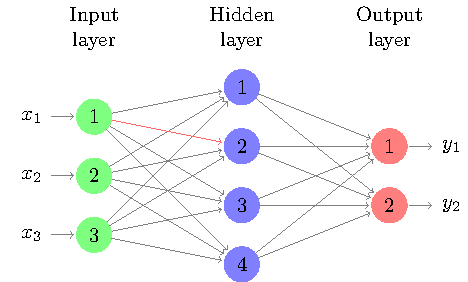
\includegraphics[scale=1.5]{images/net2.pdf}
  \caption{\label{fig:net2}Example of Neural Network with 3 layers. Here $n_1=3$, $n_2=4$ and $n_3=2$. The connection in red is denoted as $w^{(1)}_{12}$ (according to Equation ~\ref{eq:w})}
\end{figure}

Each of those connections has a weight $w$. To denote these weights we are going to use the form $w_{ij}^{(k)}$ where $k$ means which layer the connection departs from, $i$ means which neuron of layer $k$ the connection departs from and $j$ means which neuron of layer $k+1$ the connections arrives to (See Figure ~\ref{fig:net2}). Therefore $w$ is:
\begin{equation}
\begin{aligned}
  & w^{(k)}_{ij} \\
  & i=1,\dots,n_k \\
  & j=1,\dots,n_{k+1} \\
  & k=1,\dots,m
\end{aligned}
\label{eq:w}
\end{equation}\\

Each neuron has a bias that allow set how excited is a neuron. A really excited neuron always output '1' while a non-excited neuron always give us '0'. The bias helps the network to adjust some neurons as important since not every neuron output is equally interesting. The work of a single neuron is as simple as add the bias and the weighted inputs and apply a function to the result ~\cite[Chapter~27]{springer}. The output $o$ of a neuron is:
\begin{equation}
  o^{(k)}_i=
  \begin{cases}
    x_i, & k=1 \\
    f\bigg(u^{(k)}_i+\sum^{n_{k-1}}_{j=1}w^{(k-1)}_{ji}\cdot o^{(k-1)}_j\bigg), & k>1
  \end{cases}
\end{equation}
For example, for the neuron 3 in blue of Figure ~\ref{fig:net2} the output will be $o^{(2)}_3=f(u^{(2)}_3+w^{(1)}_{13}\cdot o^{(1)}_1+w^{(1)}_{23}\cdot o^{(1)}_2+w^{(1)}_{33}\cdot o^{(1)}_3)$. For the same neuron the scheme is showed in Figure ~\ref{fig:neur1}.
\begin{figure}[H]
  \center
  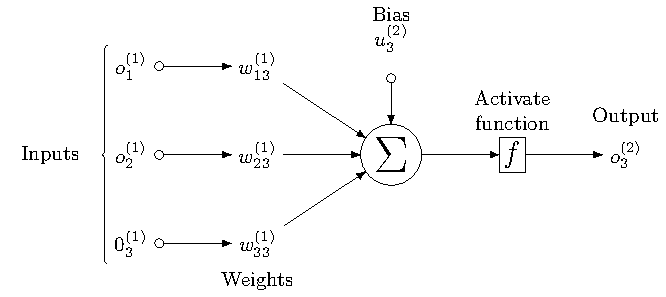
\includegraphics[scale=1]{images/neuron1.pdf}
  \caption{\label{fig:neur1}Example of the task of a single neuron \cite{neurdiag}}
\end{figure}

\section{Back Propagation}
Now a Neural Network could be programmed with all showed on \ref{sec:hood}, a program that output $y_1,$ and $y_2$ could be developed. But, where is the "learning" of deep learning here? Nowhere, yet. Is the moment of teaching the net with examples, giving it some inputs and showing it the expected outputs. The \textit{Back Propagation Algorithm} is going to achieve it. The goal of this method is to minimize the error using the method of gradient descent.

\subsection{Activation Function}
As explained before each neuron has to apply one function to the result of its computing. One of the most popular functions used for this purpose is the sigmoid:
\begin{equation}
  s(x)=\frac{1}{1+e^{-cx}}
\end{equation}
The shape of this function depends on the value of $c$, but for simplicity $c=1$ is going to be used. The derivate of the sigmoid function respect of x is $s(x)^\prime=s(x)(1-s(x))$. One of the reasons why this function is used is the simplicity of the derivate, because it allows to make all the derivates later more easily ~\cite[Chapter~7]{rojas}.
\begin{figure}
  \center
  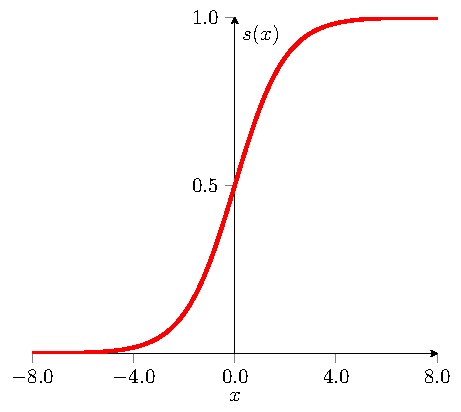
\includegraphics{images/sigmoid.pdf}
  \caption{Shape of the sigmoid with $c=1$}
\end{figure}

\subsection{The Error}
The error could be measured in differents ways. The most common and apparently most effective method is to calculate the Euclidean distance. It allows to measure the error in different dimensions, for example, the error in $\rm I\!R^1$ between $4$ and $1$ is $E=4-3=1$. For $\rm I\!R^2$ you should use the Pythagorean theorem, and for $\rm I\!R^n$ the distance is:
\begin{equation}
  E_{(p,q)}=\sqrt{(p_1-q_1)^2+(p_2-q_2)^2+\dots+(p_i-q_i)^2+\dots+(p_n-q_n)^2}
\end{equation}

Is important to know how to size the error that the net has because you have to tell the network how far was the result from the expected output. And only once you have the distance between the target and the output you can adjust the knobs to achieve a better result.

How much the knob must be changed? It depends on how important is that knob for the result. For example it might be possible that changing one knob will get the same result. In this case it does not matter if we adjust the knob, but, what about one knob that when adjusted change the result drastically? Here the new position of the knob is realy important. Hence we need the partial error with respect a specific weight or bias ~\cite[Chapter~2]{nielsen}:
\begin{equation}
  \frac{\partial e}{\partial w^{(k)}_{ij}} \quad \textrm{or} \quad \frac{\partial e}{\partial u^{(k)}_{i}}
\end{equation}

\subsection{The Correction}
Once we can calculate the error depending on one parameter we are ready to make the correction to the network. The process is simple, first you feed the input layer with some data, then you get the result and compare it with the target and finally you make this adjustment for each weight and bias (the $\alpha$ is the learning constant and represent how far is the next step in the gradient descent) ~\cite[Chapter~7]{rojas}:
\begin{equation}
\begin{aligned}
  w^{(k)}_{ij} & \Rightarrow & w^{(k)}_{ij} - \alpha \frac{\partial e}{\partial w^{(k)}_{ij}} \\
  u^{(k)}_{i} &  \Rightarrow & u^{(k)}_{i} - \alpha \frac{\partial e}{\partial u^{(k)}_{i}}
\end{aligned}
\label{eq:corr}
\end{equation}

To develop a working neural network is now possible with all this knwoledge. First we have to declare the architecture of our net. Then we set random weights and biases and we start teaching the net. Imagine you have a 10.000 images dataset, then you take 90\% of those images to train the net, and the other 10\% for testing how well we have developed it. We feed the network with one of those images from the train set and make the correction as we have seen in \ref{eq:corr}. Ideally we should do it with all the train set but as the size of that set could be (and should be) huge, we just take a small batch representative and apply the correction for each image of the batch. Once we have done it we have complete one epoch. With just one epoch the network still giving us weird answers, so what we have to do is to train the network with several epochs and then our network is trained and ready.

To measure how intelligent our network is you can use the test set of images to calculate the accuracy.

\section{Implementation}
With the full algorithm of the back propagation a full Neural Network could be developed. You can do it by following the steps and code it in \textit{Python}, \textit{Haskell}, \textit{Matlab} \dots But as you develop your net you will notice that it is only valid for a certain network architecture, and it is pretty slow because of the languages. You can develop it on \textit{C++} or even in \textit{C} what will need a lot of effort for achieving more speed.

But as Neural Networks are not new and as they are well known and famous, there are many tools you can choose for creating your model. It will be much faster to implement it and the net will run also faster since the tools are optimized. One of the most famous tools is developed by \textit{Google}. They are the kings of de big data and they are using the data for machine learning so they have created \textit{TensorFlow} carefully to fullfill all their needs.

\subsection{Tensorflow}
TensorFlow is an open source software library for numerical computation using data flow graphs. It was developed initially for \textit{Google} machine learning purposes but it could be used in other domains. It was released for the first time in 2015 and now it is on version \textit{1.4.0}. This tool gives you a APIs of different levels of abstraction that allow you to work with complex numerical computation in an abstract, easy and elegant way ~\cite{amy}.

In TensorFlow \textbf{SIN ACABAR}

\subsection{MNIST Data Set}
Every time you start learning a new language you first start with \textit{Hello World}. In the machine learning this program is the \textit{MNIST} problem. The \textit{MNIST} data set is composed by 70.000 images of handwritten digits (See Figure ~\ref{fig:mnist}), and the whole data set has been studied several times as it has shown to fit very well with basic neural networks.

\begin{figure}
  \center
  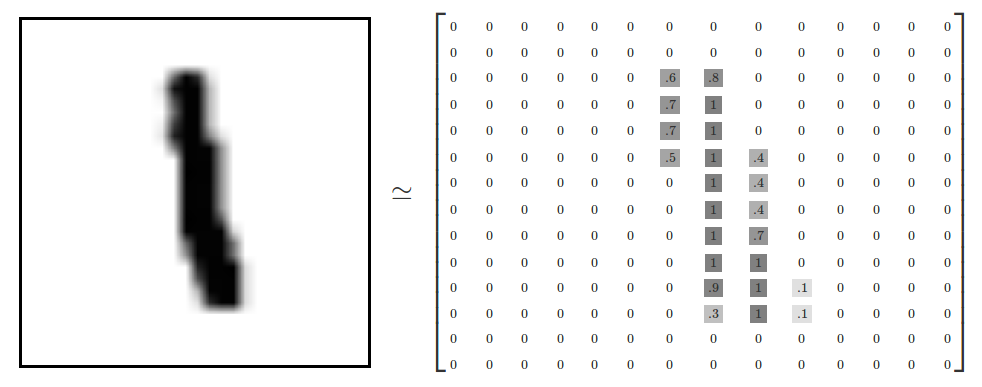
\includegraphics[scale=0.4]{images/MNIST-Matrix.png}
  \caption{The images are $28x28$ pixels where each of them describes how dark is that point of the image. This figure is $14x14$ for simplicity ~\cite{colah} }
  \label{fig:mnist}
\end{figure}

In order to be able to give the images to the input they are stored as flattened vector of $24\cdot24=784$ numbers. The output of the networ will be an array of dimension $10$ where each position is $0$ but one has the value $1$. The position of the value $1$ represents which number the network thinks the image is. For instance, if the input is the image of a $8$ the perfect output is $[0,0,0,0,0,0,0,0,1,0]$.

\subsection{Building the Model}
As we have seen from the data the input is of dimension $784$ while the output has $10$ outcoming values. We are going to have two hidden layers of 256 neurons each. We are going to define the parameters of the network so we also can define the learning constant $\alpha=0.01$, the number of epochs to $1000$ and the batch size (number of images the network train with in each epoch) to $100$.

\begin{lstlisting}[language=python]
#Network parameters
n_hidden1 = 256
n_hidden2 = 256
n_input = 784
n_output = 10
#Learning parameters
learning_constant = 0.01
number_epochs = 1000
batch_size = 100
\end{lstlisting}

We also have to specify how we are going to input the data and how we expect the ouput, for that we are goin gto define the placehoders, defining that the input is a two dimensions array of floats, one dimension is every input (784) and as we do not know the number of images we are going to give we write \textit{None} for the other dimension. In a similar way the output is defined.

\begin{lstlisting}[language=python]
X = tf.placeholder("float", [None, n_input])
Y = tf.placeholder("float", [None, n_output])
\end{lstlisting}

Each neuron has a bias and each pair of neurons of neighbours layers has a weight so we must define all of them:
\begin{lstlisting}[language=python]
#Biases first hidden layer
b1 = tf.Variable(tf.random_normal([n_hidden1]))
#Biases second hidden layer
b2 = tf.Variable(tf.random_normal([n_hidden2]))
#Biases output layer
b3 = tf.Variable(tf.random_normal([n_output]))

#Weights connecting input layer with first hidden layer
w1 = tf.Variable(tf.random_normal([n_input, n_hidden1]))
#Weights connecting first hidden layer with second hidden layer
w2 = tf.Variable(tf.random_normal([n_hidden1, n_hidden2]))
#Weights connecting second hidden layer with output layer
w3 = tf.Variable(tf.random_normal([n_hidden2, n_output]))
\end{lstlisting}

Done, we have defined $728\cdot256+256\cdot256+256\cdot10=254464$ weights in three lines, TensorFlow is powerful. To finish we just have to tell how the four layers are connected, and the the model will be ready to be trained. To achieve it we have to define what is the task for each neuron. If one vector of data $x$ is incoming to a neuron, it has to weight it ($w$) add the bias $u$ and apply the activation function $f(x\cdot W+u)$. Making the product of each input data with their weight is as simple as applying \textit{tf.matmul}, then add the bias with \textit{tf.add} and finally apply the activation function \textit{tf.nn.relu}.
\begin{lstlisting}[language=python]
#The incoming data given to the
#network is input_d
def multilayer_perceptron(input_d):
    #Task of neurons of first hidden layer
    layer_1 = tf.nn.relu(tf.add(tf.matmul(input_d, w1), b1))
    #Task of neurons of second hidden layer
    layer_2 = tf.nn.relu(tf.add(tf.matmul(layer_1, w2), b2))
    #Task of neurons of output layer
    out_layer = tf.add(tf.matmul(layer_2, w3),b3)
    return out_layer
\end{lstlisting}

The full neural network model can be stored in a single variable in such a simple way as (\textit{X} is the placeholder we have already defined as the input of the network):
\begin{lstlisting}[language=python]
# Create model
neural_network = multilayer_perceptron(X)
\end{lstlisting}
\subsection{Training the Model}
Is the moment of training the network. For that purpose we have to define what is the error and which method we are going to use to fix it. The error or the loss is calculated giving our model and the placeholder of the output. For fixing that loss we are going to apply the gradient descent optimizer and we have to define what we want to reduce and what is the learning constant.

\begin{lstlisting}[language=python]
#Define the loss or the error
loss_op = tf.reduce_mean(tf.nn.softmax_cross_entropy_with_logits(
                         logits=neural_network,labels=Y))
#Define how to fix it
optimizer = tf.train.GradientDescentOptimizer(learning_constant)
                      .minimize(loss_op)
\end{lstlisting}

Next step is iterate trought all the epochs. In each one the program should take one batch of images and their expected output, feed the network with it, and finally apply the optimizer we have already defined. The task of running the epochs could not be done in such a simple way as we have defined the model. The train should be performed inside a TensorFlow session after all the declares variables are initialized. The session allows not just declare the model but perform operations.

\begin{lstlisting}[language=python]
#Initializing the variables
init = tf.global_variables_initializer()
#Create a session
with tf.Session() as sess:
    sess.run(init)
    #Training epoch
    for epoch in range(number_epochs):
        #Get one batch of images
        batch_x, batch_y = mnist.train.next_batch(batch_size)
        #Run the optimizer feeding the network with the batch
        sess.run(optimizer, feed_dict={X: batch_x, Y: batch_y})
        #Display the epoch (just every 100)
        if epoch % 100 == 0:
            print("Epoch:", '%d' % (epoch))
\end{lstlisting}

\subsection{Evaluating the Model}
The network is already trained so it is the time of test how well we have designed it and how much it has learned. One part of the date set was reserved for testing. The outputs of the network are not as perfect as one vector with all $0$ but one $1$ pointing the solution. Actually it is more close to something like $[0.01,0.94,0.02,0.025,0.025,0.06,0.01,0.01,0.4,0.04]$ because the network is not absolutely sure about the answer so the output is something like "I am 94\% sure that this is a 1 but it could be a 8 in a 4\% and a bit percentage for the other options". To transform that answers the \textit{softmax} function should be applied. It takes the bigger number and transform it to a $1$ while change the other smallers numbers with $0$s. Now we define what is a correct answer with \textit{tf.equal}, one prediction is correct if it is equal to the expected output, easy. To finish we define the accuracy to print it and feed the network wiht the test subset.

\begin{lstlisting}[language=python]
# Test model
pred = tf.nn.softmax(neural_network)  # Apply softmax to logits
correct_prediction = tf.equal(tf.argmax(pred, 1), tf.argmax(Y, 1))
# Calculate accuracy
accuracy = tf.reduce_mean(tf.cast(correct_prediction, "float"))
print("Accuracy:", accuracy.eval({X: mnist.test.images, Y: mnist.test.labels}))
\end{lstlisting}

If we execute the code we get an accuracy close to 90\%. It might seem that is a great result, it answer correctly 9 out of 10 times. But in machine learning this result is pretty bad, it is normal because the network used is the most simple network but compared with other kind of models it is a bit shaming.

